\documentclass[10pt, twocolumn, twoside, letterpaper]{IEEEtran}
\IEEEoverridecommandlockouts

\usepackage[activate={true, nocompatibility}, final, tracking=true, kerning=true, spacing=true, factor=1100, stretch=10, shrink=10]{microtype}
\linespread{0.9}

\makeatletter
\def\ps@IEEEtitlepagestyle{
  \def\@evenfoot{}
}

% \def\ps@IEEEtitlepagestyle{
%   \def\@oddfoot{\mycopyrightnotice}
%   \def\@evenfoot{}
% }
% \def\mycopyrightnotice{
%   {\footnotesize
%   \begin{minipage}{\textwidth}
%   \centering
%   978-1-7281-7693-2/20/\$31.00 \copyright2020 IEEE
%   \end{minipage}
%   }
% }

\ifCLASSINFOpdf
   \usepackage[pdftex]{graphicx}
\else
   \usepackage[dvips]{graphicx}
\fi

\ifCLASSOPTIONcompsoc
  \usepackage[caption=false, font=normalsize, labelfont=sf, textfont=sf]{subfig}
\else
  \usepackage[caption=false, font=footnotesize]{subfig}
\fi

\usepackage{amsmath}
\usepackage{bm}
\usepackage{amssymb}
\usepackage{algorithm}
\usepackage{algorithmic}
\usepackage{stfloats}
\usepackage{url}
\usepackage{siunitx}
\usepackage{fancyref}

\usepackage{geometry}
\geometry{letterpaper, top=0.7in, bottom=0.7in, left=0.65in, right=0.65in}

\usepackage[acronym, nomain]{glossaries}

% Define "long-s" key: 
\glsaddkey* {longs}% key 
{\glsentrylong{\glslabel}s}% default value 
{\glsentrylongs}% command analogous to \glsentrytext 
{\Glsentrylongs}% command analogous to \Glsentrytext 
{\glslongs}% command analogous to \glstext 
{\Glslongs}% command analogous to \Glstext 
{\GLSlongs}% command analogous to \GLStext

%% Define "short-s" key: 
\glsaddkey* {shorts}% key 
{\glsentryshort{\glslabel}s}% default value 
{\glsentryshorts}% command analogous to \glsentrytext 
{\Glsentryshorts}% command analogous to \Glsentrytext 
{\glsshorts}% command analogous to \glstext 
{\Glsshorts}% command analogous to \Glstext 
{\GLSshorts}% command analogous to \GLStext

\DeclareRobustCommand{\glss}[1]
{%
  \ifglsused{#1}{\glsshorts{#1}}{\glslongs{#1} (\glsshorts{#1})\glsunset{#1}}%
}

\DeclareRobustCommand{\Glss}[1]
{%
  \ifglsused{#1}{\Glsshorts{#1}}{\Glslongs{#1} (\glsshorts{#1})\glsunset{#1}}%
}

\newacronym{18F-FDG}{18F-FDG}{Fluorine-$18$ Fludeoxyglucose}
\newacronym{1D}{1D}{$1$-Dimensional}
\newacronym{2D}{2D}{$2$-Dimensional}
\newacronym{3D}{3D}{$3$-Dimensional}
\newacronym[longs={$3$-Dimensional Point Clouds}, shorts={3DPCs}]{3DPC}{3DPC}{$3$-Dimensional Point Cloud}
\newacronym{4D}{4D}{$4$-Dimensional}
\newacronym{4DCT}{4DCT}{$4$-Dimensional Computed Tomography}
\newacronym[longs={Attenuation Corrections}, shorts={ACs}]{AC}{AC}{Attenuation Corrected}
\newacronym[longs={Affine Deformations}, shorts={ADs}]{AD}{AD}{Affine Deformation}
\newacronym{AP}{AP}{Anterior Posterior}
\newacronym{ATP}{ATP}{Adenosine Triphosphate}
\newacronym{BE}{BE}{Bending Energy}
\newacronym{BFGS}{BFGS}{Broyden Fletcher Goldfarb Shanno}
\newacronym[longs={B-Splines}, shorts={BSs}]{BS}{BS}{B-Spline}
\newacronym[longs={Cross Correlations}, shorts={CCs}]{CC}{CC}{Correlation Coefficient}
\newacronym{CCT}{CCT}{Cine Computed Tomography}
\newacronym{CG}{CG}{Conjugate Gradient}
\newacronym{COM}{COM}{Centre of Mass}
\newacronym[longs={Control Points}, shorts={CPs}]{CP}{CP}{Control Point}
\newacronym[longs={Control Point Grids}, shorts={CPGs}]{CPG}{CPG}{Control Point Grid}
\newacronym{CT}{CT}{Computed Tomography}
\newacronym{DDG}{DDG}{Data Driven Gating}
\newacronym{DD-PCA}{DD-PCA}{Data Driven Principal Component Analysis Surrogate Signal Extraction}
\newacronym{DD}{DD}{Data Driven}
\newacronym[longs={Deformation Vector Fields}, shorts={DVFs}]{DVF}{DVF}{Deformation Vector Field}
\newacronym{EANM}{EANM}{European Association of Nuclear Medicine}
\newacronym{EM}{EM}{Expectation Maximisation}
\newacronym{FDG}{FDG}{Fluorodeoxyglucose}
\newacronym{FFT}{FFT}{Fast Fourier Transform}
\newacronym[longs={Fields of View}, shorts={FOVs}]{FOV}{FOV}{Field Of View}
\newacronym{FWHM}{FWHM}{Full Width at Half Maximum}
\newacronym{GAN}{GAN}{Generative Adversarial Networks}
\newacronym{GD}{GD}{Gradient Descent}
\newacronym{GE}{GE}{General Electric}
\newacronym[longs={Ground Truths}, shorts={GTs}]{GT}{GT}{Ground Truth}
\newacronym{HU}{HU}{Hounsfield Unit}
\newacronym[longs={Image Registrations}, shorts={IRs}]{IR}{IR}{Image Registration}
\newacronym{KBq/mL}{KBq/mL}{Kilo Becquerel per Millilitre}
\newacronym{KeV}{KeV}{Kilo Electron Volt}
\newacronym{KRG}{KRG}{Kinetic Respiratory Gating}
\newacronym{KV}{KV}{Kilo Volt}
\newacronym{L-BFGS-B}{L-BFGS-B}{Low memory Broyden Fletcher Goldfarb Shanno Bounded}
\newacronym{L-BFGS}{L-BFGS}{Low memory Broyden Fletcher Goldfarb Shanno}
\newacronym[longs={Light Emitting Diodes}, shorts={LEDs}]{LED}{LED}{Light Emitting Diode}
\newacronym{LE}{LE}{Linear Energy}
\newacronym{LR}{LR}{Linear Regression}
\newacronym[longs={Lines of Responses}, shorts={LORs}]{LOR}{LOR}{Line of Response}
\newacronym[longs={Mean Absolute Errors}, shorts={MAEs}]{MAE}{MAE}{Mean Absolute Error}
\newacronym{MAD}{MAD}{Median Absolute Difference}
\newacronym{MAPE}{MAPE}{Mean Absolute Percentage Error}
\newacronym{MBF}{MBF}{Myocardial Blood Flow}
\newacronym{MCIR}{MCIR}{Motion Compensated Image Reconstruction}
\newacronym[longs={Motion Compensated Images}, shorts={MCIs}]{MCI}{MCI}{Motion Compensated Image}
\newacronym{MC}{MC}{Motion Correction}
\newacronym{MIC}{MIC}{Medical Imaging Convention}
\newacronym{MI}{MI}{Mutual Information}
\newacronym{ML}{ML}{Maximum Likelihood}
\newacronym{MLAA}{MLAA}{Maximum Likelihood Reconstruction of Activity and Attenuation}
\newacronym{MLE}{MLE}{Maximum Likelihood Estimation}
\newacronym{MLEM}{MLEM}{Maximum Likelihood Expectation Maximisation}
\newacronym[longs={Motion Models}, shorts={MMs}]{MM}{MM}{Motion Model}
\newacronym[longs={Myocardial Perfusion Images}, shorts={MPIs}]{MPI}{MPI}{Myocardial Perfusion Imaging}
\newacronym{MR}{MR}{Magnetic Resonance}
\newacronym{MSc}{MSc}{Master of Science}
\newacronym{MSE}{MSE}{Mean Squared Error}
\newacronym[longs={Attenuation Maps}, shorts={Mu-Maps}]{Mu-Map}{Mu-Map}{Attenuation Map}
\newacronym[longs={Non-Attenuation Corrections}, shorts={NACs}]{NAC}{NAC}{Non-Attenuation Corrected}
\newacronym{NMI}{NMI}{Normalised Mutual Information}
\newacronym{ND}{ND}{$n$-Dimensional}
\newacronym{NMC}{NMC}{Non-Motion Corrected}
\newacronym{NN}{NN}{Neural Network}
\newacronym[longs={Non-Rigid Deformations}]{NRD}{NRD}{Non-Rigid Deformation}
\newacronym{NTOF}{NTOF}{Non-Time-of-Flight}
\newacronym{OSEM}{OSEM}{Ordered Subset Expectation Maximisation}
\newacronym[longs={Principal Components}, shorts={PCs}]{PC}{PC}{Principal Component}
\newacronym{PCA}{PCA}{Principal Component Analysis}
\newacronym{PCC}{PCC}{Pearson Correlation Coefficient}
\newacronym{PET}{PET}{Positron Emission Tomography}
\newacronym{PLL}{PLL}{Poisson Log Likelihood}
\newacronym{PSD}{PSD}{Power Spectral Density}
\newacronym{PSMA}{PSMA}{Prostate Specific Membrane Antigen}
\newacronym{RANSAC}{RANSAC}{Random Sample Consensus}
\newacronym[longs={Respiratory Correspondence Models}, shorts={RCMs}]{RCM}{RCM}{Respiratory Correspondence Model}
\newacronym[longs={Rigid Deformations}, shorts={RDs}]{RD}{RD}{Rigid Deformation}
\newacronym{RDP}{RDP}{Relative Difference Prior}
\newacronym{RM}{RM}{Respiratory Motion}
\newacronym{RMC}{RMC}{Respiratory Motion Correction}
\newacronym{RMSE}{RMSE}{Root Mean Square Error}
\newacronym[longs={Regions of Interest}, shorts={ROIs}]{ROI}{ROI}{Region of Interest}
\newacronym{RPM}{RPM}{Real Time Position Management}
\newacronym{RTPM}{RTPM}{Real Time Position Management}
\newacronym{SAM}{SAM}{Spectral Analysis Method}
\newacronym{SGD}{SGD}{Stochastic Gradient Descent}
\newacronym{SI}{SI}{Superior Inferior}
\newacronym{SIRF}{SIRF}{Synergistic Image Reconstruction Framework}
\newacronym[longs={Signal to Noise Ratios}, shorts={SNRs}]{SNR}{SNR}{Signal to Noise Ratio}
\newacronym[longs={Surrogate Signals}, shorts={SSs}]{SS}{SS}{Surrogate Signal}
\newacronym{SSD}{SSD}{Sum of Squared Differences}
\newacronym{STFT}{STFT}{Short-time Fourier transform}
\newacronym{STIR}{STIR}{Software for Tomographic Image Reconstruction}
\newacronym[longs={Standard Uptake Values}, shorts={SUVs}]{SUV}{SUV}{Standard Uptake Value}
\newacronym{SVD}{SVD}{Singular Value Decomposition}
\newacronym{TOF}{TOF}{Time-of-Flight}
\newacronym[longs={Thin Plate Splines}, shorts={TPSs}]{TPS}{TPS}{Thin Plate Spline}
\newacronym{XCAT}{XCAT}{$4$-Dimensional Extended Cardiac Torso}


\usepackage[style=ieee, doi=false, isbn=false, url=false, maxbibnames=1, minbibnames=1, maxcitenames=1, mincitenames=1, backend=biber, defernumbers=false]{biblatex}
\addbibresource{./bibtex/bib/Biblio.bib}

\AtEveryBibitem{\clearfield{month}}
\AtEveryBibitem{\clearfield{day}}
\AtEveryBibitem{\clearfield{volume}}
\AtEveryBibitem{\clearfield{issue}}
\AtEveryBibitem{\clearfield{pages}}
\AtEveryBibitem{\clearfield{number}}
\AtEveryBibitem{\clearfield{title}}
\AtEveryBibitem{\clearfield{isbn}}
\AtEveryBibitem{\clearfield{keywords}}
\AtEveryBibitem{\clearfield{issn}}
\AtEveryBibitem{\clearfield{journal}}

\begin{document}

\title{Comparison of Motion Modelling Motion Correction Methods For PET/CT Using a Single Breath Hold Attenuation Map}

\pagestyle{plain}
\pagenumbering{gobble}

\author{
    \IEEEauthorblockN{
        Alexander~C.~Whitehead~\IEEEauthorrefmark{1}~\IEEEauthorrefmark{2},
        Kuan-Hao~Su~\IEEEauthorrefmark{3},
        Scott~W.~Wollenweber~\IEEEauthorrefmark{3},
        Charles~W.~Stearns~\IEEEauthorrefmark{3},
        Brian~F.~Hutton~\IEEEauthorrefmark{1},
        Jamie~R.~McClelland~\IEEEauthorrefmark{2} and
        Kris~Thielemans~\IEEEauthorrefmark{1}~\IEEEauthorrefmark{2}
    }
    
    \IEEEauthorblockA{
        \IEEEauthorrefmark{1}
        \textit{Institute of Nuclear Medicine, University College London, UK}
    }
    
    \IEEEauthorblockA{
        \IEEEauthorrefmark{2}
        \textit{Centre for Medical Image Computing, University College London, UK}
    }
    
    \IEEEauthorblockA{
        \IEEEauthorrefmark{3}
        \textit{Molecular Imaging and Computed Tomography Engineering, GE Healthcare, USA}
    }
        
    \vspace{-1.0cm}

    \thanks{This research is supported by GE Healthcare, the NIHR UCLH Biomedical Research Centre and the UCL EPSRC Centre for Doctoral Training in Intelligent, Integrated Imaging in Healthcare (i4health) grant (EP/L016478/1). The software used was partly produced by the Computational Collaborative Project on Synergistic Biomedical Imaging, CCP SyneRBI, UK EPSRC grant (EP/T026693/1).}%
    \thanks{Jamie~R.~McClelland is supported by a Cancer Research UK Centres Network Accelerator Award grant (A21993) to the ART-NET consortium and a CRUK Multi-disciplinary grant (CRC 521).}%
    \thanks{(contact: \texttt{alexander.whitehead.18@ucl.ac.uk}).}%
}

\maketitle
\IEEEpeerreviewmaketitle

\begin{abstract}
    It is increasingly becoming apparent that the introduction of motion models into respiratory motion correction methods is a technique that can lead to a further reduction in blurring and artefacts. However, the pool of research where motion modelling methods are applied to positron emission tomography with a computed tomography attenuation map is relatively shallow. Previous work has presented methods through which non-attenuation corrected time-of-flight data can be used to fit motion models, not only to motion correct the volumes themselves, but also to warp a single attenuation map to the positions of the initial gated data. This work seeks to extend previous work to offer a comparison of respiratory motion correction methods, not only with and without motion models but also to compare pair-wise and group-wise registration techniques on simulation data with a low count rate, including randoms and scatter, where the attenuation map is from a pseudo breath hold acquisition. To test this $4$-Dimensional Extended Cardiac Torso data is simulated and reconstructed without attenuation correction, then motion corrected using one of pair-wise, pair-wise with motion model, group-wise and group-wise with motion model registration. Next these motion corrected volumes are registered to the breath hold attenuation map and the resultant deformation vector fields are composed for each method. The attenuation map can thus be deformed to the position of the gates using the inverse of these deformations. With the deformed attenuation maps an attenuation corrected reconstruction can be performed and motion correction applied, again, using the relevant method. Evaluation is carried out between the results, as well as against a non-motion corrected example, using a visual analysis, a comparison of profiles through a lesion inserted into the data as well as standard uptake values. Results indicate that the incorporation of a motion model vastly improves contrast and quantification of these noisy volumes, as well as that group-wise provides similar effects when compared to pair-wise registration, but to a lesser degree.
\end{abstract}

\vspace{-0.4cm}

% \vspace{-0.5cm}

\section{Introduction} \label{sec:introduction}
    \IEEEPARstart{M}{otion} modelling is a \gls{MC} technique, where time- or gate-dependence of \glss{DVF} are parameterised in terms of a \gls{SS}~\cite{McClelland2013}. \glss{MM} attempt to improve upon solely registering data, being more robust to noise, but also allow for the correction of unseen data. It has shown good promise in \gls{CT}~\cite{Li2007EnhancedModel}, \gls{MR}~\cite{Manke2002RespiratoryModels}
    and  combined \gls{PET}/\gls{MR}~\cite{Manber2016JointCorrection.}, but has not yet seen widespread adoption in clinical \gls{PET}, where \gls{PET}/\gls{CT} is far more common.
    
    \gls{RM} reduces resolution and degrades the accuracy of quantification in \gls{PET} by introducing blurring to the \gls{PET} volume and also misalignment between the \gls{PET} and \gls{CT}~\cite{Nehmeh2008a}. Most existing \gls{MC} methods rely on pair-wise registration of gated \gls{PET} volumes, this is a challenging problem due to the low contrast and high noise~\cite{Oliveira2014}. Respiratory \gls{MC} is an ideal problem area for the application of \glss{MM} as \glss{SS} are already commonly available from respiratory gating, such as acquired by \gls{RPM} or \gls{PCA}~\cite{Thielemans2011}.
    
    In previous work, the possibility of using \glss{MM} to \gls{MC} \gls{NAC} \gls{TOF} \gls{PET}, and warp a \gls{Mu-Map} from a position close to the mean respiratory position to each gate, was investigated. It was found that the combination of both the \gls{MM} and \gls{TOF} was sufficient to perform an \gls{AC} reconstruction with \gls{MC}, without introducing artefacts, while increasing resolution and quantification accuracy~\cite{Whitehead2019ImpactPET},~\cite{Whitehead2020PET/CTFields}. This work seeks to extend the method further through the use of a more modular framework, which allows for the fair comparison of different registration methods, both with and without \glss{MM}. Furthermore, this work uses more realistic simulation and count levels, compared to previous work (where more simple registration methods would fail). Additionally, this work strives to improve the \gls{Mu-Map} warping aspect of the previous method, by fixing the \gls{Mu-Map} at end inhalation (as opposed to the mean respiratory position). This is more clinically relevant but also challenging.
    
    A method incorporating \glss{MM} for dynamic \gls{PET}/\gls{CT}, was proposed and tested on clinical data in~\cite{Chan2018Non-RigidPET}. The work presented here, differentiates itself by firstly using a \gls{2D} \gls{SS}, rather than a \gls{1D} \gls{SS}, thus both inter- and intra-gate motion can be included in the model, at the expense that each gate contains fewer counts. Additionally, the group-wise method, presented here, makes use of an iterative \gls{MC} algorithm rather than using only a pair-wise method.

% \vspace{-0.3cm}

\section{Methods} \label{sec:methods}
    \subsection{XCAT Volume Generation} \label{sec:xcat_volume_generation}
        \gls{XCAT}~\cite{Segars2010} was used to generate $240$ volumes over a \SI{120}{\second} period using a respiratory trace, derived from \gls{MR} navigator patient data. The max displacement of \acrlong{AP} and \acrlong{SI} motion, was set to \SI{1.2}{\centi\metre} and \SI{2.0}{\centi\metre} respectively. Activity concentrations were derived from a static \gls{18F-FDG} patient scan. The \gls{FOV} included the base of the lungs, diaphragm and the top of the liver with a \SI{20}{\milli\metre} diameter spherical lesion (smaller than the max displacement, due to \gls{RM}) was placed into the base of the right lung (within the max displacement, due to \gls{RM}, of the diaphragm).
    
    % \vspace{-0.3cm}
    
    \subsection{PET Acquisition Simulation and Non-Attenuation Corrected Image Reconstruction} \label{sec:pet_acquisition_simulation_and_non_attenuation_corrected_image_reconstruction}
        \gls{PET} acquisitions were simulated (and reconstructed) using \gls{STIR}~\cite{Thielemans2012, Nikos2019} through \gls{SIRF}~\cite{Ovtchinnikov2017}, to forward project data using the geometry of a \gls{GE} Discovery $710$, but using a \gls{TOF} resolution of \SI{375}{\pico\second}. This \gls{TOF} resolution is higher than that of the $710$, but is closer to the newer \gls{GE} Signa \gls{PET}/\gls{MR} system. \gls{TOF} mashing was used to reduce computation time resulting in $13$ \gls{TOF} bins of size \SI{376.5}{\pico\second}. Attenuation was included using the relevant \glss{Mu-Map} generated by \gls{XCAT}. Pseudo-randoms and scatter were added. Randoms were added by summing the scaled mean value to each voxel of each volume prior to forward projection. Pseudo scatter was added by summing the scaled and smoothed mean \gls{Mu-Map} prior to forward projection, the smoothing parameter was optimised to give scatter which tapered at the same rate as in clinical data. A full scatter simulation was not performed due to software limitations.
        
        Noise was simulated, such that data matched an acquisition over \SI{120}{\second}, emulating a standard single bed position acquisition. The count rate was selected to match that of research scans, i.e. below that of diagnostic clinical scans. This count rate was selected as a 'worst case scenario'.
        
        A respiratory \gls{SS} was generated using \gls{PCA}~\cite{Thielemans2011}. The magnitude of this signal and its gradient, was used to gate data into $30$ respiratory bins using displacement gating ($10$ amplitude and $3$ gradient bins). Gates with fewer than $0.42$\% of the counts were discarded. For the purpose of the \gls{MM} fitting, \gls{SS} values were determined for the post-gated data by taking an average of the \gls{SS} values of data in each bin.
        
        Data were reconstructed, without \gls{AC}, using \gls{OSEM} with two full iterations and $24$ subsets~\cite{Hudson1994}.
    
    % \vspace{-0.3cm}
    
    \subsection{Registration} \label{sec:registration}
        Before being registered, each volume underwent pre-processing. Including replication of end-slices, transformation to be approximately normally distributed~\cite{Johnson2013} and post-smoothing. This pre-processing was only applied to intermediate data and was not used for the final output of the method.% Initially, because a breath hold \gls{Mu-Map} is the final target position for the \gls{MC} $10$ repeating slices are added to the top and bottom of each volume to allow space for the volumes to be registered into. First, the mean value was subtracted from each volume and then each voxel in the volume was divided by the standard deviation of the volume. Next a Yeo-Johnson transformation~\cite{Johnson2013} was applied to transform data to be more Gaussian like, this acted as a pseudo histogram normalisation. Finally data underwent Gaussian smoothing.
        
        Two registration methods were examined in this work. Firstly, pair-wise registration, where the reference position was selected as the gate with the highest number of counts. All other gates were registered to it. Secondly, group-wise registration, where after an initial pair-wise registration step, the \glss{DVF} generated had the inverse mean of all \glss{DVF} composed with them, before a new reference volume was resampled. Registration to the new reference volume, followed by the inverse mean composition and resample, continued for a set number of iterations. NiftyReg~\cite{Modat2010} was used to perform registrations using a B-spline parameterisation. The Gaussian smoothing \gls{FWHM}, \acrlong{CPG} spacing of the B-spline coefficients, \acrlong{BE} regularisation term weight and number of iterations were tuned using a grid search.
    
    % \vspace{-0.3cm}
    
    \subsection{Motion Model Estimation} \label{sec:motion_model_estimation}
        If a \gls{MM} was used, then it was fit as a direct \acrlong{RCM} on the \glss{DVF} from~\Fref{sec:registration} and the \gls{SS} from~\Fref{sec:pet_acquisition_simulation_and_non_attenuation_corrected_image_reconstruction}. A weighted \acrlong{LR} was used, where the weighting was taken based on the number of counts in each gate. Once a \gls{MM} was fit, new \glss{DVF} were generated for each gate, using the \gls{SS} values used to fit the \gls{MM}. For group-wise registration, \gls{MM} fitting occurred between iterations, the \glss{DVF} generated by the \gls{MM} were used to resample the new target volume at each iteration.
    
    % \vspace{-0.3cm}
    
    \subsection{Attenuation Map Warping} \label{sec:attenuation_map_warping}
        A \gls{Mu-Map} at end inhalation was selected from the \glss{Mu-Map} generated by \gls{XCAT}. The \gls{PET} volume from the previous step was then registered to this \gls{Mu-Map}, and the resulting \glss{DVF} were composed with the \glss{DVF} from the last iteration of the \gls{MC} method, and a new volume resampled. The inverse of these \glss{DVF}, were then used to warp the \gls{Mu-Map} to each gate.
    
    % \vspace{-0.3cm}
    
    \subsection{Motion Corrected Image Reconstruction with AC} \label{sec:attenuation_corrected_image_reconstruction}
        Data were re-reconstructed with \gls{AC}, using the \glss{Mu-Map} from~\Fref{sec:attenuation_map_warping}. The same reconstruction parameters as in~\Fref{sec:attenuation_corrected_image_reconstruction} were used. \gls{MC} was then applied to data following~\Fref{sec:registration},~\Fref{sec:motion_model_estimation} and~\Fref{sec:attenuation_map_warping}. Volumes were post-filtered using a Gaussian smoothing, with a \gls{FWHM} of \SI{6.39}{\milli\metre} in the transverse plane (equivalent to three voxels) and \SI{3.27}{\milli\metre} (equivalent to one voxel) in the axial direction.
    
    % \vspace{-0.3cm}
    
    \subsection{Evaluation} \label{sec:evaluation}
        In addition to the reconstructions performed in~\Fref{sec:attenuation_corrected_image_reconstruction}, data were also reconstructed without \gls{MC}, using either a sum of all \glss{Mu-Map} (to emulate an \gls{AV-CCT}), or the end inhalation \gls{Mu-Map}. For the present evaluation, the volumes without \gls{MC} were registered to the position of the end inhalation \gls{Mu-Map}. Additionally, \glss{DVF} generated by each method were also applied to noiseless data for visual analysis.
        
        Comparisons used included: A profile over the lesion, \gls{SUV}\textsubscript{max} and \gls{SUV}\textsubscript{peak} (defined following \gls{EANM} guidelines~\cite{Boellaard2015FDG2.0}).

% \vspace{-0.3cm}

\section{Results} \label{sec:results}
    \begin{figure}
        % \vspace{-0.0cm}
        
        \centering
        
        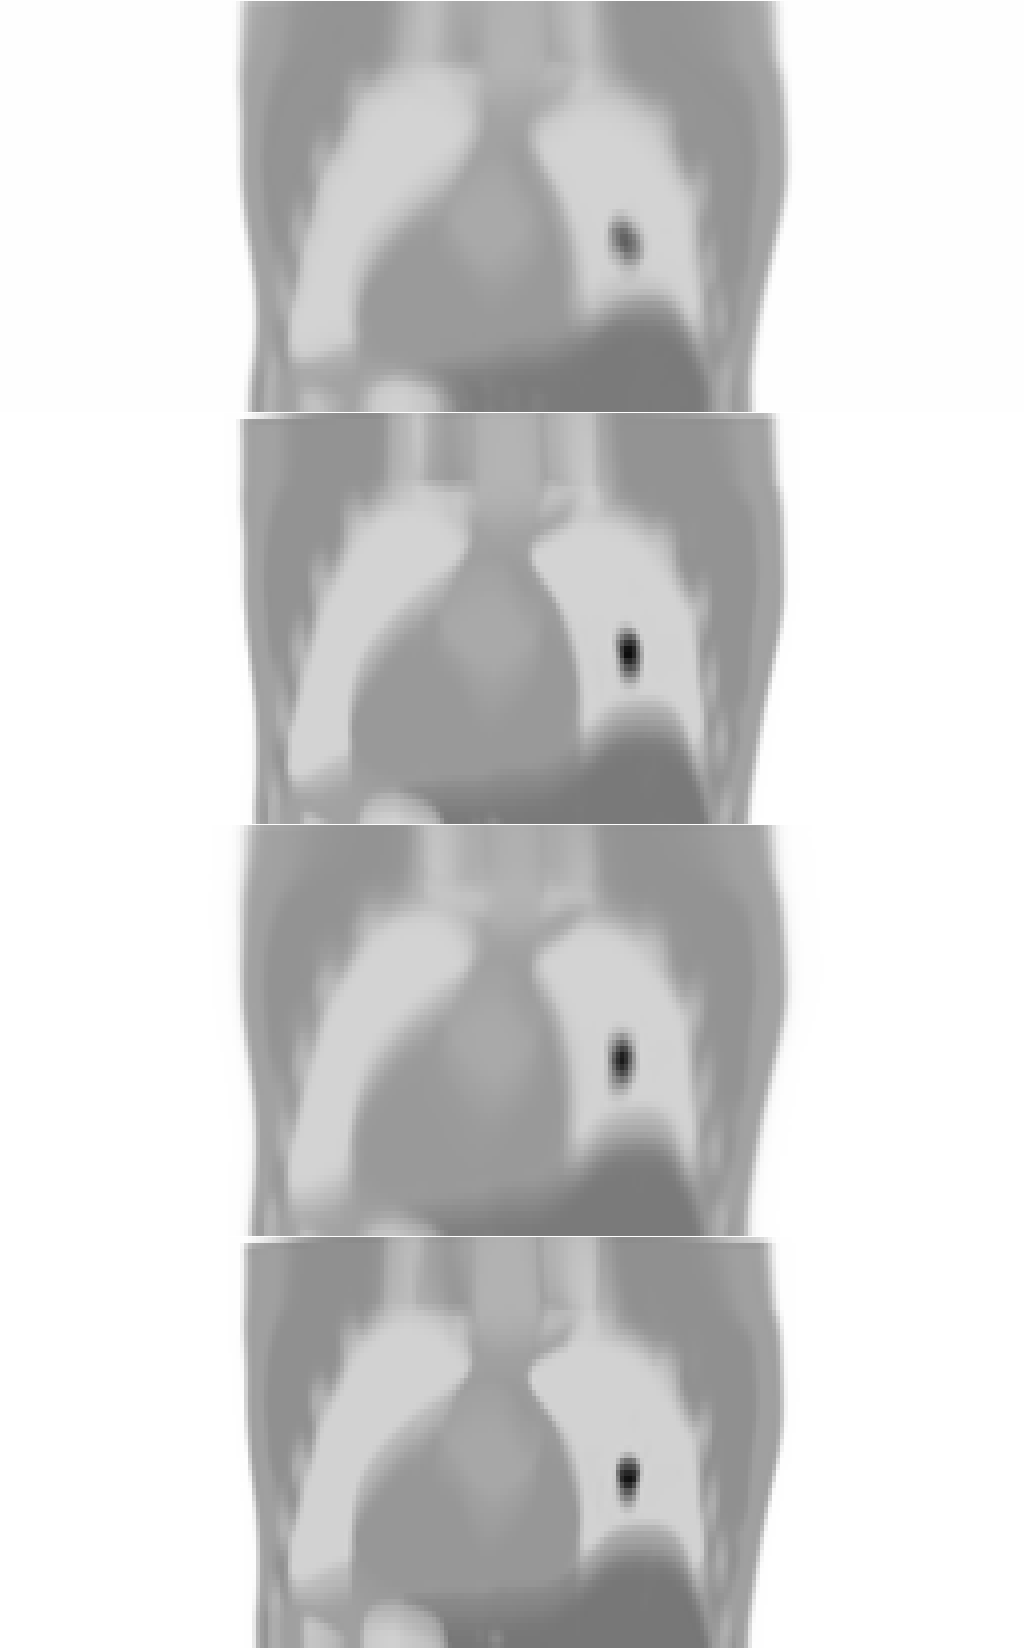
\includegraphics[width=1.0\linewidth]{figures/visual_analysis.png}
        
        % \vspace{-0.3cm}
        
        \captionsetup{singlelinecheck=false, justification=centering}
        \caption{First column contains \gls{AC} \gls{MC} reconstructions and the second column contains the result of applying the final \gls{MC} on the original XCAT images (for easier assessment of the accuracy of the estimated \glss{DVF}); ungated static \gls{CT}, ungated \gls{AV-CCT}, pair-wise, pair-wise \gls{MM}, group-wise, group-wise \gls{MM}. Colour map ranges are consistent for all images in each column.}
        
        \label{fig:visual_analysis}
        
        % \vspace{-0.3cm}
    \end{figure}
    
    \begin{figure}
        % \vspace{-0.0cm}
        
        \centering
        
        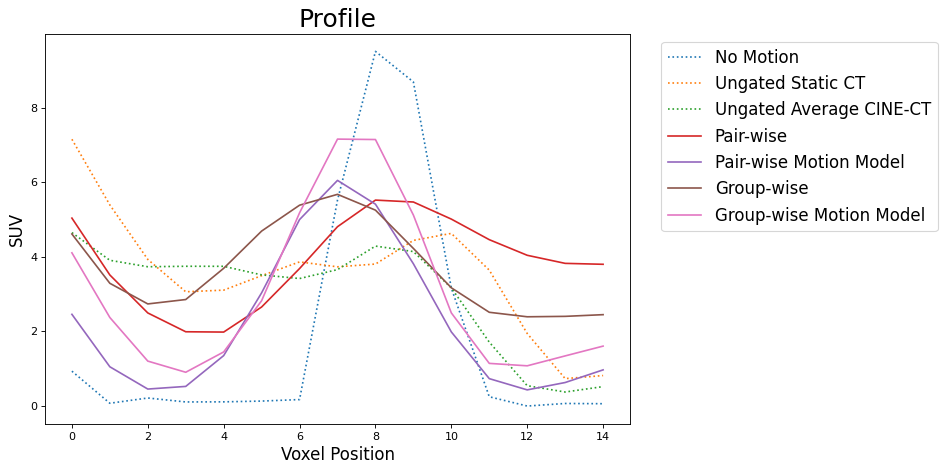
\includegraphics[width=1.0\linewidth]{figures/profile.png}
        
        % \vspace{-0.3cm}
        
        \captionsetup{singlelinecheck=false, justification=centering}
        \caption{A profile across the lesion for; ungated static \gls{CT}, ungated \gls{AV-CCT}, pair-wise, pair-wise \gls{MM}, group-wise, group-wise \gls{MM}.}
        
        \label{fig:profile}
        
        % \vspace{-0.5cm}
    \end{figure}
    
    \begin{table}
        \centering
        
        \captionsetup{singlelinecheck=false, justification=centering}
        \caption{Comparison of \gls{SUV}\textsubscript{max} and \gls{SUV}\textsubscript{peak} between: ungated static \gls{CT}, ungated \gls{AV-CCT}, pair-wise, pair-wise \gls{MM}, group-wise, group-wise \gls{MM}.}
        
        \resizebox*{1.0\linewidth}{!}
        {
            \begin{tabular}{||c|cc||}
                \hline
                \textbf{\gls{SUV}}                  & \textbf{Max}  & \textbf{Peak} \\
                \hline
                \textbf{No Motion}                  & $9.50$        & $9.06$ \\
                \hline
                \textbf{Ungated Static \gls{CT}}    & $5.25$        & $5.15$ \\
                \textbf{Ungated \gls{AV-CCT}}       & $5.38$        & $5.07$ \\
                \hline
                \textbf{Pair-wise}                  & $4.21$        & $3.92$ \\
                \textbf{Pair-wise \gls{MM}}         & $6.63$        & $6.07$ \\
                \hline
                \textbf{Group-wise}                 & $4.42$        & $4.21$ \\
                \textbf{Group-wise \gls{MM}}        & $7.64$        & $7.03$ \\
                \hline
            \end{tabular}
        }
        \label{tab:suv}
        
        % \vspace{-0.5cm}
    \end{table}
    
    A visual comparison of the reconstructed images (see ~\Fref{fig:visual_analysis}) shows that more blurring can be seen at the boundary between the diaphragm and lung for the \gls{MM} free methods. Additionally, where a \gls{MM} was used, the lesion appears to be more homogeneous.
     
    The peak of the profile (see~\Fref{fig:profile}) is greater for \gls{MM} methods than for \gls{MM} free methods. However, the peaks for all \gls{MC} methods are greater than ungated methods.
     
    \gls{SUV} results consistently show that including \glss{MM} increases the \gls{SUV} when compared to when one is not used (see~\Fref{tab:suv}).

% \vspace{-0.3cm}

\section{Discussion and Conclusions} \label{sec:discussion_and_conclusions}
    Results from a visual analysis, a comparison of profiles and \gls{SUV}, show that adding a \gls{MM} to any \gls{MC} method (tested here) improved the quality of volumes produced. Although, from a visual analysis volumes appear preferable with any \gls{MC} method, quantitative evaluation points to the conclusion that for \gls{MC} to be successful, for very noisy data, \glss{MM} are required in practice.
    
    In the future, work will focus on incorporating the methods presented here into an iterative \acrlong{IR} and \gls{MC} method and tested on patient data from several research studies.% It may also be of interest to consider the impact that robust regression methods have on fitting a \gls{MM}, such as using a robust objective function or fitting the \gls{MM} indirectly on the eigenvectors of applying \gls{PCA} to the initial \glss{DVF}.
    

\vspace{-0.4cm}

\AtNextBibliography{\scriptsize}
\printbibliography

\end{document}
